\chapter{Lista de Componentes e Análise de Custos}
\label{ch:custos}

\section{Lista de componentes}
A tabela~\ref{tab:bom} apresenta a lista de componentes do protótipo, com os preços unitários consultados em lojas online em novembro de 2026. Os preços com fonte indicada foram confirmados na loja; os restantes, assinalados com (E), são estimativas para componentes genéricos. Os valores em libras e dólares foram convertidos aproximadamente para euros e não incluem portes.

\begin{table}[H]
\centering\small
\caption{Lista de componentes e custo do protótipo.}
\begin{tabularx}{\textwidth}{>{\raggedright\arraybackslash}p{4.4cm}c>{\raggedright\arraybackslash}Yrr}
\toprule
Componente & Qtd. & Fonte do preço & Unit. (€) & Total (€)\\\midrule
\multicolumn{5}{l}{\textit{Processamento, sensores e comunicação}}\\
NUCLEO-F767ZI & 1 & TME \cite{tmenucleo} (s/ IVA) & 35,00 & 35,00\\
Módulo GY-85 (9 eixos) & 1 & Hobby Electronica \cite{gy85} & 20,95 & 20,95\\
Módulo Bluetooth modo duplo (HM-12) & 1 & Bot'n Roll \cite{hm12} & 12,90 & 12,90\\
\multicolumn{5}{l}{\textit{Atuação}}\\
Servo TowerPro MG996R & 2 & Waveshare \cite{waveshareMG996R} & 4,60 & 9,20\\
\multicolumn{5}{l}{\textit{Alimentação e segurança}}\\
Bateria LiPo 2S \SI{2200}{\milli\ampere\hour} & 1 & (E) & 20,00 & 20,00\\
\acrshort{ubec} \SI{6}{\volt} & 1 & FlyingTech \cite{flyingtechubec} & 10,00 & 10,00\\
Regulador \textit{buck} \SI{5}{\volt} & 1 & (E) & 4,00 & 4,00\\
Interruptor basculante DPST (corte dos servos) & 1 & (E) & 5,00 & 5,00\\
Fusível e porta-fusível & 1 & (E) & 2,00 & 2,00\\
Interruptor geral & 1 & (E) & 1,00 & 1,00\\
Condensador, resistências, \acrshort{led} & -- & (E) & 2,00 & 2,00\\
\multicolumn{5}{l}{\textit{Mecânica}}\\
Filamento PLA (cerca de \SI{400}{\gram}) & -- & (E) & 8,00 & 8,00\\
Parafusos M2, M3 e M4, porcas e anilhas & -- & (E) & 8,00 & 8,00\\
Cabos e conectores (XT60, Dupont) & -- & (E) & 5,00 & 5,00\\
\midrule
\multicolumn{4}{l}{\textbf{Total do protótipo}} & \textbf{143,05}\\
\bottomrule
\end{tabularx}
\label{tab:bom}
\end{table}

Ficam de fora da tabela o equipamento de laboratório (osciloscópio, multímetro, impressora 3D), que já existe, e alguns acessórios recomendados que não fazem parte do protótipo: um carregador balanceado para baterias LiPo e um saco de proteção para a carga, com um custo estimado de 25~€ e 8~€, respetivamente.

\acompletar{preços efetivamente pagos, se forem diferentes}

\section{Análise de custos}
O custo total estimado do protótipo é de cerca de 143~€, abaixo do limite de 150~€ definido no requisito RNF9. A figura~\ref{fig:custos} mostra a distribuição do custo por grupo.

\begin{figure}[H]
\centering
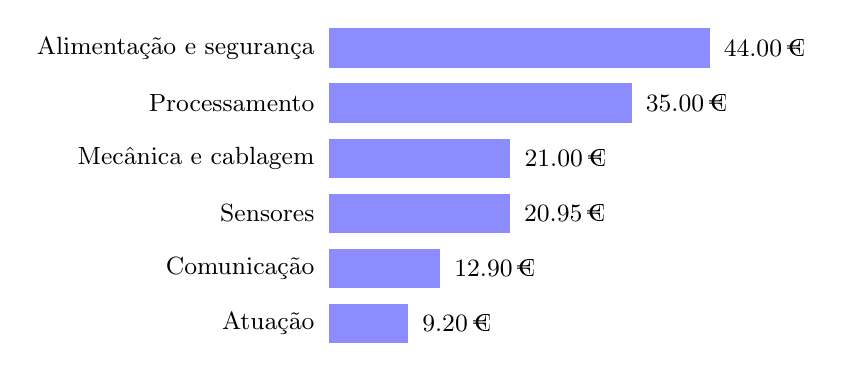
\begin{tikzpicture}[x=0.11cm]
\foreach \lab/\val/\pos in {Alimentação e segurança/44.00/0, Processamento/35.00/1, Mecânica e cablagem/21.00/2, Sensores/20.95/3, Comunicação/12.90/4, Atuação/9.20/5}{
  \node[anchor=east, font=\small] at (0,-\pos*0.7) {\lab};
  \fill[blue!45] (0.5,-\pos*0.7-0.25) rectangle (0.5+\val,-\pos*0.7+0.25);
  \node[anchor=west, font=\small] at (1+\val,-\pos*0.7) {\val\,€};
}
\end{tikzpicture}
\caption{Distribuição do custo do protótipo por grupo.}
\label{fig:custos}
\end{figure}

A alimentação e a segurança representam o maior grupo (cerca de 31\,\% do total), mais do que o processamento. Isto resulta de a bateria e os reguladores terem de ser dimensionados para os picos de corrente dos servos e de se ter incluído desde o início um interruptor de corte dos servos e proteção por fusível. A placa de desenvolvimento é o componente individual mais caro (25\,\%), seguida do GY-85 (15\,\%). Os sensores e os atuadores, que são o núcleo funcional do sistema, custam em conjunto cerca de 21\,\%.

A troca da MPU6050 pelo GY-85 aumentou o custo em cerca de 15~€. Uma segunda \gls{imu} na base, para a compensação antecipativa, acrescentaria outro tanto se fosse também um GY-85 e levaria o total acima dos 150~€; para essa função bastaria um sensor de seis eixos mais barato, já que o magnetómetro não é necessário.

Se o sistema viesse a ser produzido em série, o custo por unidade poderia baixar bastante. A placa NUCLEO seria substituída por uma placa de circuito impresso própria, apenas com o microcontrolador e os componentes necessários, ou por um microcontrolador mais simples, já que o estudo do estado da arte mostrou que um filtro complementar e dois \gls{pid} não exigem um Cortex-M7. Um microcontrolador com Bluetooth integrado, como o ESP32-S3, eliminaria também o módulo de comunicação. Em contrapartida, um produto comercial teria custos que um protótipo não tem, como o projeto da placa, os ensaios de conformidade descritos no capítulo~\ref{ch:seguranca} e a embalagem.

\acompletar{horas de trabalho da equipa, se se pretender incluir o custo de engenharia}
